%! TEX root = ../../master.tex
\lecture[Beweis des allgemeinen Liftungsssatzes. Charakteristische Untergruppe einer Überlagerung (an einem Punkt). Homöomorphe Überlagerungen. Injektivität von $p_*$. Klassifikation der zusammenhängenden Überlagerungen der  $S^1$. Semilokal einfachzusammenhängende Räume.  Universelle Überlagerungen. Existenzsatz für universelle Überlagerungen.]{Di 22 Jun 2021}{Charakteristische Untergruppen}

\begin{lemma*}\label{lm:hilfslemma:wege-mit-gleichem-endpunkt-werden-auf-gleiche-endpunkte-geliftet}
    Betrachte die gleiche Situation wie im vorherigem Satz. Seien $w$, $w'$ zwei Wege in $Y$ mit Anfangspunkt  $y_0$ und gleichem Endpunkt. Dann ist
    \[
        L(f \circ  w,e_0)(1) = L(f \circ w',e_0)(1)
    .\] 
\end{lemma*}

\begin{proof}
    Die Verknüpfung $w \star \overline{w'}$ ist eine Schleife an $y_0$. Dann ist $f\circ (w \star \overline{w'})$ eine Schleife an $x_0$ und
    \[
        [f \circ (w\star \overline{w'})] \in f_*(\pi_1(Y,y_0)) \subset p_*(\pi_1(E,e_0))
    .\] 

Sei $\tilde{w}$ eine Schleife in $E$ an  $e_0$, so dass $p \circ  \tilde{w}$ homotop ist zu $f \circ  (w \star \overline{w'}) = (f \circ  w) \star ( f \circ  \overline{w'})$ relativ Endpunkten.

Also ist auch relativ Endpunkten:
\[
    (p \circ  \tilde{w}) \star (f \circ  w') \simeq (f \circ  w) \star (f \circ  \overline{w'}) \star (f \circ  w') \simeq f \circ  w
.\] 

Nun ist
\[
    (p \circ  \tilde{w}) \star (f \circ  w') = p \circ (\tilde{w} \star L(f \star w', e_0))
.\] 
und
\[
    f \circ  w \simeq p \circ  L(f \circ  w,e_0)
.\] 
Nach dem \nameref{thm:homotopieliftungssatz} ist somit $\tilde{w} \star L(f \circ  w', e_0)$ homotop (in $E$) zu  $L(f \circ  w, e_0)$ relativ Endpunkten. Insbesondere haben die beiden Wege den gleichen Endpunkt. Also
\[
    L(f \circ  w, e_0)(1) = \tilde{w} \star L(f \circ  w', e_0)(1) = L(f \circ  w', e_0)
.\] 

\end{proof}

\begin{proof}[Fortsetzung des Beweises von \autoref{thm:allgemeiner-liftungssatz}]
    Nun konstruieren wir uns die Hebung von $Y$ nach  $E$. Definiere  $\tilde{f}$ punktweise, indem wir für $y\in Y$ einen Weg $w$ von  $y_0$ nach $y$ wählen (denn  $Y$ ist nach Voraussetzung wegzusammenhängend), und dann
    \[
        \tilde{f}(y) \coloneqq  L(f\circ w, e_0)(1)
    .\] 
    setzen. Als erstes müssen wir prüfen, dass diese Definition wohldefiniert ist, d.h. $\tilde{f}(y)$ ist unabhängig von der Wahl von $y$. Das haben wir aber gerade genau in \autoref{lm:hilfslemma:wege-mit-gleichem-endpunkt-werden-auf-gleiche-endpunkte-geliftet} gesehen.

    Wir prüfen, dass $\tilde{f}$ eine Hebung ist, dazu ist
    \begin{IEEEeqnarray*}{rCl}
        p(\tilde{f}(y)) & = & p(L(f \circ  w,e_0)(1)) \\
                        & = & p(L(f \circ w,e_0))(1) \\
                        & = & (f \circ w)(1) \\
                        & = & f(w(1)) = f(y)
    \end{IEEEeqnarray*}

    Es bleibt zu zeigen, dass $\tilde{f}$ stetig ist.

    \begin{claim}
        Für jedes $y\in Y$ und jede Umgebung $V$ von  $\tilde{f}(y)$ existiert eine Umgebung $W$ von  $y$ mit  $\tilde{f}(W)\subset V$, d.h. $\tilde{f}$ ist stetig.
    \end{claim}
    \begin{subproof}
        Sei $U\subset X$ eine offene Teilmenge von $X$, die  $f(y)$ enthält, und über der  $p$ trivial ist. Sei  $u\colon  p^{-1} (U) \to  U \times p^{-1} (f(y))$ ein Homöomorphismus über $p$, und setze dann  $V' \coloneqq  V \cap  u^{-1}(U \times \left \{\tilde{f}(y)\right\} )$. Es ist dann $p|_{V'}\colon  V' \to  p(V')$ eine Homöomorphismus mit  $p(V')$, einer Umgebung von  $f(y)$.

        Jetzt erhalten wir mit $f^{-1}(p(V'))$ eine Umgebung von $y$. Da  $Y$ lokal wegzusammenhängend ist, finden wir eine wegzusammenhängende Umgebung  $W\subset f^{-1}(p(V'))$. Esverbleibt zu zeigen:
    \end{subproof}

    \begin{claim}
        $\tilde{f}(W) \subset V'$, also insbesondere $\tilde{f}(y') \in V'$.
    \end{claim}

    \begin{subproof}
        Sei $y' \in W$ und $w$ ein Weg von  $y_0$ nach $y$ in  $Y$ und  $w'$ ein Weg von  $y$ nach  $y'$ in  $W$. Dann ist  $w \star w'$ ein Weg von  $y_0$ nach $y'$. Es ist 
         \begin{IEEEeqnarray*}{rCl}
             \tilde{f}(y') & = & L(f \circ (w \star w' ), e_0)(1) \\
                          & = & L(f \circ w, e_0) \star L(f \circ  w', \underbrace{L(f \circ  w, e_0)(1)}_{= \tilde{f}(y)})(1) 
         \end{IEEEeqnarray*}
         Sehen wir uns den Weg $L(f \circ  w', \tilde{f}(y))$ genauer ein, so wissen wir - weil $p|_{V'}$ ein Homöomorphismus ist - , dass
         \[
             L(f \circ  w', \tilde{f}(y)) = p|_{V'}^{-1} \circ  f \circ  w'
         .\] 
         und hat somit Bild in $V'$. Insbesondere liegt auch der Endpunkte disees Weges, also  $\tilde{f}(y')$, in $V'$.
    \end{subproof}

    Es bleibt, die Eindeutigkeit von $\tilde{f}$ zu zeigen. Ist $g$ eine weitere Hebung von  $f$, so ist $g|_W$ eine Hebung von  $f \circ w$, also ist zwingendermaßen
    \[
        g(y) = g(w(1)) = L(f \circ w, e_0)(1) = \tilde{f}(y)
    .\] 
    nach Eindeutigkeit der Weghebung, also $\tilde{f} = g$ punktweise, und somit überall.
    \[
    \begin{tikzcd}
        & & \ar{d}{p} \\
        I \ar[dashed, bend left = 20]{urr} \ar{r}{w} & Y \ar{ur}{g} \ar{r}{f} &  X
    \end{tikzcd}
    .\] 
\end{proof}

\begin{theorem}\label{thm:abbildung-von-s^n-nach-s^1-ist-homotop-zu-konstanter-abbildung-für-n-geq-2}
    Sei $n\geq 2$. Dann ist jede stetige Abbildung $f\colon  S^n \to  S^1$ homotop zu einer konstanten Abbildung.
\end{theorem}

\begin{proof}
    Da $n\geq 2$ ist, ist $\pi_1(S^n,x_0) = \left \{\star\right\} $ trivial, also insbesonder eine Untergruppe von $\exp_*(\pi_1(\R,0))$, also existiert nach dem \nameref{thm:allgemeiner-liftungssatz} ein Lift $\tilde{f}\colon  S^n \to  \R$, sodass also kommutiert:
    \[
    \begin{tikzcd}
        & \R \ar{d}{\exp } \\
        S^n \ar[dashed]{ur}{\tilde{f}} \ar[swap]{r}{f} & S^1
    \end{tikzcd}
    .\] 
    Da $\R$ zusammenziehbar (d.h. homotopieäquivalent zu $\star$, ist  $\tilde{f}$ nullhomotop (d.h. homotop zu einer konstanten Abbildung).

    Sei $H$ eine Nullhomotopie, dann ist  $\exp  \circ  H$ eine Nullhomotopie von $f$.
\end{proof}


\begin{example}['Gegenbeispiel' zum \nameref{thm:allgemeiner-liftungssatz}]
    Die Forderung, dass $Y$ lokal wegzusammenhängend ist, ist erforderlich. Wir betrachten hierzu wieder die Sinuskurive des Topologen, deren Wegzusammenhangskomponenten wir verbunden haben, und betrachten analog zur Überlagerung  $\exp \colon  \R \to  S^1$ eine, indem wir jedes Intervall $[a,a+1]$ von  $\R$ durch die Sinuskurve, und den Kreis durch vorherigen Raum ersetzen.
    \missingfigure{Überlagerung skizzieren}
    Setzen wir also $X = Y$ und  $f = \id$, so gibt es keinen Lift, wir können diesen zwar mengentheoretisch konstruieren, allerdings wird dieser nicht stetig sein.
\end{example}

\begin{restatable}[Charakteristische Untergruppe]{definition}{DefCharakteristischeUntergruppe}\label{def:charakteristische-untegruppe}
    Sei $p\colon  E \to  X$ eine Überlagerung und sei $x_0\in X, e_0\in p^{-1} (x_0)$. Dann heißt $p_*(\pi_1(E,e_0))\subset \pi_1(X,x_0)$ die \vocab{charakteristische Untergruppe}. 
\end{restatable}

\begin{oral}
    Wir haben im \nameref{thm:allgemeiner-liftungssatz} bereits gesehen, dass diese Gruppe sehr wichtig ist.
\end{oral}

\begin{restatable}{theorem}{ThmHomoeomorpheUeberlagerungen}\label{thm:äquivalenz-von-überlagerungen-über-lokal-wegzsuammenhängendem-wegzusammenhängendem-raum}
    Sei $X$ wegzusammenhängend und lokal wegzusammenhängend und betrachte zwei Überlagerungen $p\colon  E\to X$, $p' \colon  E' \to  X$, sodass $E,E'$ zusammenhängend. Sei  $x_0\in X$ mit Urbildern $e_0\in p^{-1} (x_0)$, $e_0' \in p'^{-1} (x_0)$. Dann sind äquivalent:
    \begin{enumerate}[1)]
        \item Es existiert ein Homöomorphismus der Überlegerungen, d.h. ein $f\colon  E \to  E'$ mit $f(e_0) = e_0'$, sodass folgendes kommutiert:
            \[
                \begin{tikzcd}[column sep = tiny, ampersand replacement = \&]
                E \ar{rr}{f}[swap]{\cong} \ar[swap]{dr}{p} \& \& E' \ar{dl}{p'} \\
            \& X
            \end{tikzcd}
            \]
        \item Die charakterischen Untergruppen stimmen überein, d.h.
            \[
                p_*(\pi_1(E,e_0)) = p'_*(\pi_1(E',e_0'))
            .\] 
    \end{enumerate}
\end{restatable}


\begin{warning}
    Die Bedingung 2) erfordert wirklich, dass $p_*(\pi_1(E,e_0))$, $p'_*(\pi_1(E',e_0'))$ als Untergruppen von $\pi_1(X,x_0)$ \textit{gleich} sind, nicht nur isomorph.

    Vergleiche hierzu auch \autoref{ex:zusammenhängende-überlagerungen-der-s1}. 
\end{warning}

\begin{figure}[ht]
    \centering
    \incfig{skizze-zur-aequivalenz-von-ueberlagerungen}
    \caption{Skizze zu \autoref{thm:äquivalenz-von-überlagerungen-über-lokal-wegzsuammenhängendem-wegzusammenhängendem-raum}}
    \label{fig:skizze-zur-äquivalenz-von-überlagerungen}
\end{figure}

\begin{oral}
    Man könnte auch sagen, dass 1) $\implies$ 2) Teil des allgemeinen Hebungssatzes ist, aber wir machen das trotzdem nochmal.
\end{oral}

\begin{proof}[Beweis von \autoref{thm:äquivalenz-von-überlagerungen-über-lokal-wegzsuammenhängendem-wegzusammenhängendem-raum}]
    Es ist 
    \[
        p_*(\pi_1(E,e_0)) = (p'_* \circ  f_*)(\pi_1(E,e_0)) \subset p'_*(\pi_1(E',e_0'))
    .\] 
    Analoges gilt mit $f^{-1}$, d.h. $p'_*(\pi_1(E',e_0'))\subset p_*(\pi_1(E,e_0))$ und offensichtlich sind die Abbildungen invers zueinander.

    Für die andere Richtung beobachten wir zunächst, dass $E$ ebenfalls lokal wegzusammenhängend ist (nach  \autoref{thm:überlagerung-über-lokal-wegzusammenhängendem-raum-zerfällt-in-wegzusammenhängende-komponenten-von-e}).

    Nach dem \nameref{thm:allgemeiner-liftungssatz} finden wir also eine Abbildunge $f\colon  E \to  E'$ mit $f(e_0) = e_0')$ und $p' \circ  f = p$. Analog existiert ein $g\colon  E ' \to  E$ mit $g(e_0') = e_0$ und $ p \circ  g = p'$. Es ist aber
    \[
        p \circ (g \circ  f) = (p \circ  g) \circ  f = p' \circ  f = p
    .\] 
    und  $f\circ  f(e_0) = g(e_0' ) = e_0$, also folgt aus der Eindeutigkeit der Hebung, dass $g \circ f = \id$. Da $\id_E$ aber auch eine Hebung von  $p\colon  E \to X$ ist, folgt bereits $g \circ  f = \id_E$, und analog $f \circ  g = \id_{E'}$. Also sind $f,f'$ Homöomorphismen.
\end{proof}

\begin{restatable}{theorem}{ThmKonjugierteCharakteristischeUntergruppen}\label{thm:charakteristische-untergruppen-innerhalb-der-faser-sind-nur-konjugiert-wenn-weg-zwischen-urbildern-existiert}
    Sei $p\colon  E \to  X$ eine Überlagerung mit $x_0\in X, e_0,e_0' \in p^{-1} (x_0)$ sowie $w\colon  I \to  E$ ein Weg von $e_0$ nach $e_0'$. Dann ist
    \[
        p_*(\pi_1(E,e_0)) = [p \circ  w] \star p_*(\pi_1(E,e_0')) \star [p \circ  \overline{w}]
    .\] 
\end{restatable}

\begin{remark*}
    Die Aussage des Satzes ist so zu verstehen, dass die beiden Gruppen $p_*(\pi_1(E,e_0))$ und $p_*(\pi_1(E,e_0'))$ als \textit{Untergruppen} von $\pi_1(X,x_0)$ zueinander konjugiert sind mittels des Isomorphismus
        \begin{equation*}
        \varphi : \left| \begin{array}{c c l} 
            p_*(\pi_1(E,e_0)) & \longrightarrow & p_*(\pi_1(E,e_0')) \\
            \left[v\right] & \longmapsto &  \left[p \circ  w\right] \star \left[v\right] \star \left[p \circ  \overline{w}\right]
        \end{array} \right.
    \end{equation*}
Insbesondere sind sie also isomorph.
\end{remark*}


\begin{corollary}\label{cor:wegzusammenhängende-überlagerungen-besitzt-bis-auf-konjugation-eindeutige-charakteristische-untergruppe}
    Ist $p\colon E\to X$ eine Überlagerung mit $E$ wegzusammenhängend, so hängt  $p_*(\pi_1(E,e_0))$ nur bis auf Konjugation von der Wahl von $e_0$ ab.
\end{corollary}

\begin{proof}[Beweis vom Satz]
    Wir wissen, dass die Abbildung
        \begin{equation*}
        \begin{array}{c c l} 
            \pi_1(E,e_0') & \longrightarrow & \pi_1(E,e_0) \\
            \left[v\right] & \longmapsto &  \left[w \star v \star \overline{w}\right]
        \end{array}
    \end{equation*}
    ein Isomorphismus ist. Im Wesentlichen wenden wir nun einfach $\pi_1$ (bzw. $p_*$) auf diesen an, hierzu ist: 
    \begin{IEEEeqnarray*}{rCl}
        p_*[ w \star v \star \overline{w}] & = & [p \circ  (w \star v \star \overline{w})] \\
                                           & = & [(\underbrace{p \circ  w}_{\substack{\text{Schleife} \\ \text{in $x_0$}}}) \star (p \circ v) \star (\underbrace{p \circ  \overline{w}}_{\substack{\text{Schleife}\\\text{in $x_0$}} })] \\
                                           & = & [p \circ  w] \star [p \circ  v] \star [p \circ  \overline{w}]
    \end{IEEEeqnarray*}
    beachte, dass nun die $\star$ in der letzten Zeile die Verknüpfung in der Fundamentalgruppe  $\pi_1(X,x_0)$ bezeichnet.
\[
    p_*(\pi_1(E,e_0)) = [p \circ  w] \star p_*(\pi_1(E,e_0')) \star [p \circ  \overline{w}]
.\] 

\end{proof}

\begin{theorem}\label{thm:morphismus-von-fundamentalgruppen-bei-überlagerung-ist-trivial}
    Sei $p\colon  E \to  X$ eine Überlagerung, $x_0\in X$, $e_0\in p^{-1} (X)$. Dann ist die Abbildung
    \[
        p_*\colon  \pi_1(E,e_0) \to  \pi_1(X,x_0)
    .\] 
    injektiv.
\end{theorem}

\begin{proof}
    Für Injektivität genügt es (nach bekannter Gruppentheorie) zu zeigen, dass der Kern trivial ist.

Sei $[w]\in \pi_1(E,e_0)$. Angenommen, $[p \circ  w] = 1 \coloneqq [c_{x_0}]\in \pi_1(X,x_0)$. Sei $H$ eine Homotopie von  $p \circ  w$ nach $c_{x_0}$. Es ist $p \circ  c_{e_0} = c_{x_0}$, also $c_{e_0}$ ein Lift von $c_{x_0}$ mit gleichem Anfangspunkt wie $w$.

Nach dem \nameref{thm:homotopieliftungssatz} gibt es eine Homotopie von $w$ nach  $c_{e_0}$ relativ Endpunkten, diese Homotopie zeigt uns also genau, dass
\[
    [w] = [c_{e_0}]  = 1 \in \pi_1(E,e_0)
.\] 
und somit ist $\ker p_*$ trivial.
\end{proof}

\begin{example}[Zusammenhängende Überlagerungen der $S^1$]\label{ex:zusammenhängende-überlagerungen-der-s1}
    Wir wollen die zusammenhängenden Überlagerungen der $S^1$ bestimmen, hierzu machen wir uns zu Nutze, dass $S^1$ wegzusammenhängend und lokal wegzusammenhängend ist, sodass wir  \autoref{thm:äquivalenz-von-überlagerungen-über-lokal-wegzsuammenhängendem-wegzusammenhängendem-raum} anwenden können.

    Wir erhalten also, dass zwei solche Überlagerungen $E\to S^1$ genau dann homöomorph (über $S^1$) sind, wenn die zugehörigen charakteristischen Untergruppen (an Punkten aus der Faser von $1\in S^1$) identisch sind. Diese sind aber stets Untergruppen von $\pi_1(S^1,1) = \Z$, also klassifizieren wir diese:

    Die Untergruppen von $\Z$ sind genau $\left \{0\right\} $ (die triviale Gruppe) sowie die Gruppen $n\Z$ für $n\geq 1$. Wir erhalten in der Tat
    \begin{itemize}
        \item Für $\left \{0\right\} $ die Überlagerung $\exp \colon  \R \to  S^1$, hier hat $\R$ die charakteristische Untergruppe $p_*(\pi_1(\R,0)) = \left \{0\right\} $.
        \item Für $n\Z$ die Überlagerung
                \begin{equation*}
                    ()^k : \left| \begin{array}{c c l} 
                S^1 & \longrightarrow & S^1 \\
                z & \longmapsto &  z^k
                \end{array} \right.
            \end{equation*}
        Diese induziert den Gruppenhomomorphismus
            \begin{equation*}
            \begin{array}{c c l} 
                \pi_1(S^1,1) = \Z & \longrightarrow & \pi_1(S^1,1) = \Z \\
            1 & \longmapsto &  n
            \end{array}
        \end{equation*}
        und hat somit charakteristische Untergruppe $n\Z\subset \Z$.

        Man beachte, dass all diese charakteristischen Untergruppen für verschiedene $n$ zueinander \textit{isomorph} sind, nicht jedoch \textit{gleich}, weswegen uns \autoref{thm:äquivalenz-von-überlagerungen-über-lokal-wegzsuammenhängendem-wegzusammenhängendem-raum} auch nicht sagt, dass sie homöomorph sind.
    \end{itemize}
    Als Beispiel fällt einem noch die Überlagerung
        \begin{equation*}
            ()^{-k} : \left| \begin{array}{c c l} 
        S^1 & \longrightarrow & S^1 \\
        z & \longmapsto &  z^{-k}
        \end{array} \right.
    \end{equation*}
    ein, die  $\Z \to  \Z$ mit $1 \mapsto -n$ induziert, also keinen der vorherigen Morphismen. Die charakteristische Fundamentalgruppe ist aber ebenfalls  $n\Z$, also muss diese Überlagerung nach \autoref{thm:äquivalenz-von-überlagerungen-über-lokal-wegzsuammenhängendem-wegzusammenhängendem-raum} homöomorph zu $()^k$ sein. In der Tat ist auch
        \begin{equation*}
        \begin{array}{c c l} 
        S^1 & \longrightarrow & S^1 \\
        z & \longmapsto &  \overline{z}
        \end{array}
    \end{equation*}
    ein solcher Homöomorphismus $S^1 \stackrel{\cong}{\longrightarrow} S^1$ der Überlagerungen, denn es kommutiert:
    \[
        \begin{tikzcd}[column sep = tiny]
            S^1 \ar{rr}{z \mapsto \overline{z}}[swap]{\cong} \ar{dr}[swap]{z \mapsto z^k}& & S^1 \ar{dl}{z \mapsto z^{-n}} \\
                                                                                         & S^1
    \end{tikzcd}
    .\] 
\end{example}

\section{Die universelle Überlagerung}

Im Folgenden Kapitel widmen wir uns dem Ziel für 'schöne' Räume ein \textit{universelle} Überlagerung, d.h. eine mit $E$ einfach zusammenhängend, zu konstruieren, um die Anwendung von \autoref{thm:fundamentalgruppe-durch-überlagerung-mit-einfach-zusammenhängendem-raum} zu ermöglichen.


\begin{definition}[Semilokal einfachzusammenhängend]\label{def:semilokal-einfachzusammenhängend}
    Ein Raum $X$ heißt  \vocab{semilokal einfachzusammenhängend}, wenn $X$ lokal wegzusammenhängend ist und es für jeden Punkt  $x\in X$ eine wegzusammenhängende Umgebung $U$ von  $x$ gibt, so dass die Abbildung
    \[
        ι_* \colon  \pi_1(U,x) \to  \pi_1(X,x)
    .\] 
    trivial ist, wobei $ι\colon  U \to  X$ die kanonische Einbettung ist.
\end{definition}

\begin{remark}
    Es genügt für die Definition, $\pi_1(U,x) = 0$ oder $\pi_1(X,x) = 0$ zu haben, aber das ist nicht gefordert.
\end{remark}

\begin{example}\label{ex:hawaiian-earring}
    Intuitiv schließt obige Definition aus, dass es an $x$ immer kleinere Schleifen gibt. Ist das nämlich nicht der Fall, so gibt es in einer Umgebung keine, weswegen obige Abbildung trivial ist. Zwar könnte es in der Umgebung Schleifen  \textit{in $U$} geben, die nicht trivial sind, diese sind aber in $X$ nullhomotop.

    Der \vocab{Hawaiianische Ohrring} ist ein typisches Beispiel für einen nicht semilokal einfachzusammenhängenden Raum, weil er genau obige Intuition verletzt.

    \begin{minipage}{\textwidth}
        \centering
    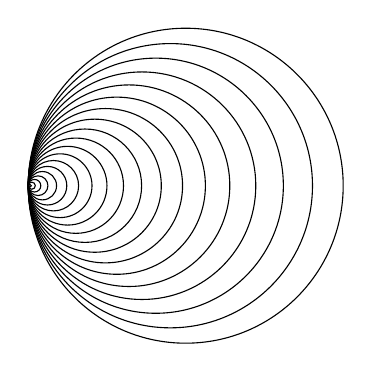
\begin{tikzpicture}
        \foreach \x in {1,...,20} {
            \draw (\x^2/200,0) circle (\x^2/200);
        }
    \end{tikzpicture}
    \captionof{figure}{Hawaiianischer Ohrring}
    \end{minipage}
\end{example}

\begin{definition}[Universelle Überlagerung]\label{def:universelle-überlagerung}
    Sei $X$ wegzusammenhängend und lokal wegzusammenhängend. Eine Überlagerung  $p\colon  E \to X$ heißt \vocab{universell}, falls $E$ einfachzusammenhängend ist. 
\end{definition}

\begin{example}
    Die Überlagerung  $\R \stackrel{\exp }{\longrightarrow} S^1$ ist eine universelle Überlagerung, denn $\R$ ist einfach zusammenhängend.
\end{example}


\begin{restatable}{theorem}{ThmUniverselleUeberlagerung}\label{thm:universelle-überlagerungen-existieren-genau-für-semilokal-einfachzusammenhängende-lokal-wegzusammenhängenden-zusammenhängende-räume}
    Sei $X$ lokal wegzusammenhängend und zusammenhängend. Dann sind äquivalent:
\begin{enumerate}[1)]
        \item $X$ ist semilokal einfachzusammenhängend.
        \item  $X$ hat eine universelle Überlagerung
        \item Für jeden Basispunkt  $x_0\in X$ und jede Untergruppe $H\subset \pi_1(X,x_0)$ existiert eine wegzusammenhängende Überlagerung $p\colon  E \to  X$ mit $e_0\in p^{-1} (x_0)$, so dass $p_*(\pi_1(E,e_0)) = H$.
    \end{enumerate}
\end{restatable}

\begin{proof}
    '$3)\implies 2)$' ist einfach ein Spezialfall, indem wir $H = \left \{0\right\} $ als die triviale Untergruppe wählen, denn dann ist $p_*(\pi_1(E,e_0)) = \left \{0\right\} $, und wir wissen bereits nach \autoref{thm:fundamentalgruppe-durch-überlagerung-mit-einfach-zusammenhängendem-raum} dass $p_*$ injektiv ist, also ist bereits $\pi_1(E,e_0) = \left \{0\right\} $, und somit ist $E$ einfach zusammenhängend.

    '$2) \implies 1)$': Sei $p\colon  E \to X$ eine universelle Überlagerung, d.h. $E$ ist einfach zusammenhängend.

    Sei  $x\in X$ und wähle $e\in p^{-1} (x)$ sowie eine offene Umgebung $V$ von  $e$, sodass  $p|_V\colon V \to  p(V)$ ein Homöomorphismus ist und $p(V)\subset X$ offen. Wähle eine wegzusammenhängende Umgebung von $x$. Die Inklusion  $U\to  X$ faktorisiert nun als
    \[
        U \to  p(V) \stackrel{p|_V^{-1}}{\longrightarrow} V \to  E \stackrel{p}{\longrightarrow} X
    .\] 
    Also erhalten wir mit $\pi_1$, dass auch
    \[
    \begin{tikzcd}
        \pi_1(U,x) \ar[bend right = 30,swap]{rr}{ι_*}\ar{r} & \underbrace{\pi_1(E,e)}_{=0} \ar{r}{p_*} & \pi_1(X,x)
    \end{tikzcd}
    .\] 
    kommutiert, was sicherlich die triviale Abbildung ist, da wir über die triviale Gruppe faktorisieren.
\end{proof}

